% =====================================================================
%  Transmissão de preços do leite entre regiões brasileiras
%  FORMATO ANPEC — Encontro Nacional de Economia
%  Normas: até 20 páginas (incl. referências/anexos); A4; Times New Roman 12;
%  espaço simples; margens >= 1,5 cm laterais e >= 2 cm sup./inf.; 1ª página com
%  título, resumo+abstract, palavras-chave+keywords, classificação JEL e área.
%  VERSÃO ANÔNIMA (avaliação cega): NÃO inclua nomes/instituições/agradecimentos.
%  Compilar com pdfLaTeX (rodar 2x para referências cruzadas).
% =====================================================================
\documentclass[12pt,a4paper]{article}

\usepackage[utf8]{inputenc}
\usepackage[T1]{fontenc}
\usepackage[brazil]{babel}
\usepackage{mathptmx}            % fonte tipo Times New Roman (texto e matemática)
\usepackage[a4paper,margin=2.5cm]{geometry}
\usepackage{setspace}
\singlespacing                   % ANPEC: espaço simples (troque por \onehalfspacing se necessário)

% --- cores (carregar xcolor[table] cedo) ---
\usepackage[dvipsnames,table]{xcolor}

% --- gráficos ---
\usepackage{graphicx}
\graphicspath{{figuras/}}

% --- pacotes exigidos pelas tabelas do kableExtra ---
\usepackage{booktabs}
\usepackage{longtable}
\usepackage{array}
\usepackage{multirow}
\usepackage{wrapfig}
\usepackage{float}
\usepackage{colortbl}
\usepackage{pdflscape}
\usepackage{threeparttable}
\usepackage{threeparttablex}
\usepackage[normalem]{ulem}
\usepackage{makecell}

% --- matemática, legendas, links ---
\usepackage{amsmath,amssymb}
\usepackage{caption}
\captionsetup{font=small,labelfont=bf}
% Float "Quadro" com numeração própria
\usepackage{newfloat}
\DeclareFloatingEnvironment[fileext=loq,listname={Lista de Quadros},name=Quadro,placement=!ht]{quadro}
\usepackage[hidelinks]{hyperref}

\setlength{\parindent}{1.25cm}
\setlength{\parskip}{0pt}

% ===== Comando de título (sem autores na versão cega) =================
\newcommand{\artigotitulo}{Transmissão de Preços do Leite ao Produtor entre Regiões Brasileiras: cointegração, correção de erro, assimetria e modelos com limiar (TVECM)}
\newcommand{\artigotituloen}{Farm-gate Milk Price Transmission across Brazilian Regions: cointegration, error correction, asymmetry and threshold models (TVECM)}

\begin{document}
\thispagestyle{empty}

% ===== PRIMEIRA PÁGINA (padrão ANPEC) ================================
\begin{center}
  {\large\bfseries \artigotitulo}\\[6pt]
  {\bfseries \artigotituloen}
\end{center}
\vspace{0.4em}

% --- Na versão NÃO anônima, descomente e preencha o bloco de autores:
% \begin{center}
%   Nome do Autor\,\footnote{Instituição, e-mail.} \quad
%   Nome do Coautor\,\footnote{Instituição, e-mail.}
% \end{center}

\begin{spacing}{1.0}
\noindent\textbf{Resumo.} Este artigo investiga a integração e a transmissão espacial
de preços do leite ao produtor entre as principais regiões do Brasil, usando dados
mensais do CEPEA/ESALQ-USP (janeiro de 2016 a abril de 2026) deflacionados pelo IPCA.
Empregam-se testes de raiz unitária, cointegração de Johansen e Phillips-Ouliaris,
modelos de correção de erro (ECM) e suas extensões assimétrica e com limiar
--- cointegração M-TAR e VECM com limiar (TVECM), que capta a banda de não-arbitragem
associada a custos de transação ---, além de causalidade de Granger e funções de
impulso-resposta. Os resultados indicam mercados fortemente integrados, com
elasticidades de longo prazo próximas da unidade, correção de erro rápida (15\% a 46\%
ao mês), transmissão majoritariamente simétrica e evidência de efeito de limiar em
pares selecionados. A referência nacional e os grandes estados produtores lideram o
descobrimento de preços.

\smallskip
\noindent\textbf{Palavras-chave:} transmissão de preços; cointegração; mercado do leite;
VECM com limiar; integração espacial.

\noindent\textbf{Classificação JEL:} Q13; Q11; C32.

\noindent\textbf{Área ANPEC:} Área 11 --- Economia Agrícola e do Meio Ambiente.
\hfill{\footnotesize\itshape (confirmar a numeração/área vigente no edital do ano)}

\medskip
\noindent\textbf{Abstract.} This paper examines the integration and spatial transmission
of farm-gate milk prices across the main Brazilian regions, using monthly CEPEA/ESALQ-USP
data (January 2016 to April 2026) deflated by the IPCA. We apply unit-root tests,
Johansen and Phillips-Ouliaris cointegration, error-correction models (ECM) and their
asymmetric and threshold extensions --- M-TAR cointegration and the threshold VECM
(TVECM), which captures the band of non-arbitrage arising from transaction costs ---,
together with Granger causality and impulse-response analysis. Results point to strongly
integrated markets, with long-run elasticities close to unity, fast error correction
(15\% to 46\% per month), mostly symmetric transmission, and evidence of threshold
effects in selected pairs. The national benchmark and the large producing states lead
price discovery.

\smallskip
\noindent\textbf{Keywords:} price transmission; cointegration; milk market; threshold
VECM; spatial integration.

\noindent\textbf{JEL Classification:} Q13; Q11; C32.
\end{spacing}

\vspace{0.6em}
\hrule
\vspace{0.8em}

% =====================================================================
\section{Introdução}
A pergunta central é dupla: (i) os mercados regionais compartilham um equilíbrio de
longo prazo (Lei do Preço Único)? e (ii) como choques de preço se propagam entre eles
--- com que velocidade, em que direção e de forma simétrica ou assimétrica? A resposta
tem implicações para a eficiência do mercado, a formação de políticas de preços agrícolas
e a compreensão do poder de mercado ao longo da cadeia do leite.

A análise segue o arcabouço clássico da literatura de transmissão de preços agrícolas:
testes de raiz unitária, cointegração de Engle-Granger e Johansen, modelos de correção
de erro (ECM), suas extensões assimétricas e de limiar --- cointegração com limiar M-TAR
e VECM com limiar (TVECM), que captura a \emph{banda de não-arbitragem} decorrente de
custos de transação. Causalidade de Granger e funções de impulso-resposta de um VAR
completam o quadro.

% =====================================================================
\section{Dados e tratamento}
Utiliza-se o Indicador CEPEA/ESALQ-USP do preço do leite ao produtor, na definição de
\emph{preço líquido médio} (efetivamente recebido pelo produtor, líquido de frete e
tributos), por ser a série contínua ao longo de todo o período. Mantêm-se apenas as
regiões com cobertura completa (jan/2016--abr/2026); Ceará e Mato Grosso do Sul foram
excluídos por terem séries interrompidas. Os preços são deflacionados pelo IPCA
(número-índice do IBGE, obtido via API do IPEA) e expressos a preços do último mês;
trabalha-se com o logaritmo natural. O Quadro~\ref{quad:fonte} resume a fonte e as
variáveis; a Tabela~\ref{tab:descritiva} traz as estatísticas descritivas.

\begin{quadro}[!h]
\centering
\caption{\label{quad:fonte}Fonte e variáveis.}
\centering
\fontsize{10}{12}\selectfont
\begin{tabular}[t]{>{\raggedright\arraybackslash}p{4cm}>{\raggedright\arraybackslash}p{11cm}}
\toprule
Item & Descrição\\
\midrule
\textbf{\cellcolor{gray!10}{Fonte}} & \cellcolor{gray!10}{CEPEA/ESALQ-USP --- Indicador do preço do leite ao produtor}\\
\textbf{Variável} & Preço líquido médio recebido pelo produtor (R\$/litro)\\
\textbf{\cellcolor{gray!10}{Frequência / Período}} & \cellcolor{gray!10}{Mensal --- jan/2016 a abr/2026 (124 observações)}\\
\textbf{Regiões} & Média Brasil + 8 estados (BA, ES, GO, MG, PR, RJ, SC, SP)\\
\textbf{\cellcolor{gray!10}{Deflator}} & \cellcolor{gray!10}{IPCA --- número-índice (IBGE, via API do IPEA); preços reais}\\
\textbf{Transformação} & Logaritmo natural (coeficientes $\approx$ elasticidades)\\
\bottomrule
\end{tabular}
\end{quadro}

\begin{table}[!h]
\centering
\caption{\label{tab:descritiva}Estatísticas descritivas do preço real do leite (R\$/litro).}
\centering
\fontsize{10}{12}\selectfont
\begin{tabular}[t]{lrrrrr}
\toprule
\textbf{Região} & \textbf{Média} & \textbf{Desv.-padrão} & \textbf{Mínimo} & \textbf{Máximo} & \textbf{CV (\%)}\\
\midrule
\cellcolor{gray!10}{Bahia} & \cellcolor{gray!10}{2,293} & \cellcolor{gray!10}{0,455} & \cellcolor{gray!10}{1,580} & \cellcolor{gray!10}{3,407} & \cellcolor{gray!10}{19,8}\\
Espírito Santo & 2,318 & 0,517 & 1,618 & 4,085 & 22,3\\
\cellcolor{gray!10}{Goiás} & \cellcolor{gray!10}{2,465} & \cellcolor{gray!10}{0,585} & \cellcolor{gray!10}{1,399} & \cellcolor{gray!10}{4,400} & \cellcolor{gray!10}{23,7}\\
Média Brasil & 2,457 & 0,530 & 1,519 & 4,230 & 21,6\\
\cellcolor{gray!10}{Minas Gerais} & \cellcolor{gray!10}{2,497} & \cellcolor{gray!10}{0,540} & \cellcolor{gray!10}{1,555} & \cellcolor{gray!10}{4,272} & \cellcolor{gray!10}{21,6}\\
Paraná & 2,477 & 0,535 & 1,510 & 4,208 & 21,6\\
\cellcolor{gray!10}{Rio de Janeiro} & \cellcolor{gray!10}{2,433} & \cellcolor{gray!10}{0,541} & \cellcolor{gray!10}{1,512} & \cellcolor{gray!10}{4,010} & \cellcolor{gray!10}{22,2}\\
Santa Catarina & 2,393 & 0,532 & 1,437 & 4,200 & 22,2\\
\cellcolor{gray!10}{São Paulo} & \cellcolor{gray!10}{2,508} & \cellcolor{gray!10}{0,515} & \cellcolor{gray!10}{1,655} & \cellcolor{gray!10}{4,146} & \cellcolor{gray!10}{20,5}\\
\bottomrule
\end{tabular}
\end{table}


Os níveis médios são próximos entre as regiões (R\$~2,29 a R\$~2,51/litro) e os
coeficientes de variação são semelhantes ($\approx 20$--$24\%$), um primeiro indício de
que os mercados se movem de forma articulada (Figuras~\ref{fig:series} e \ref{fig:spreads}).

\begin{figure}[H]\centering
  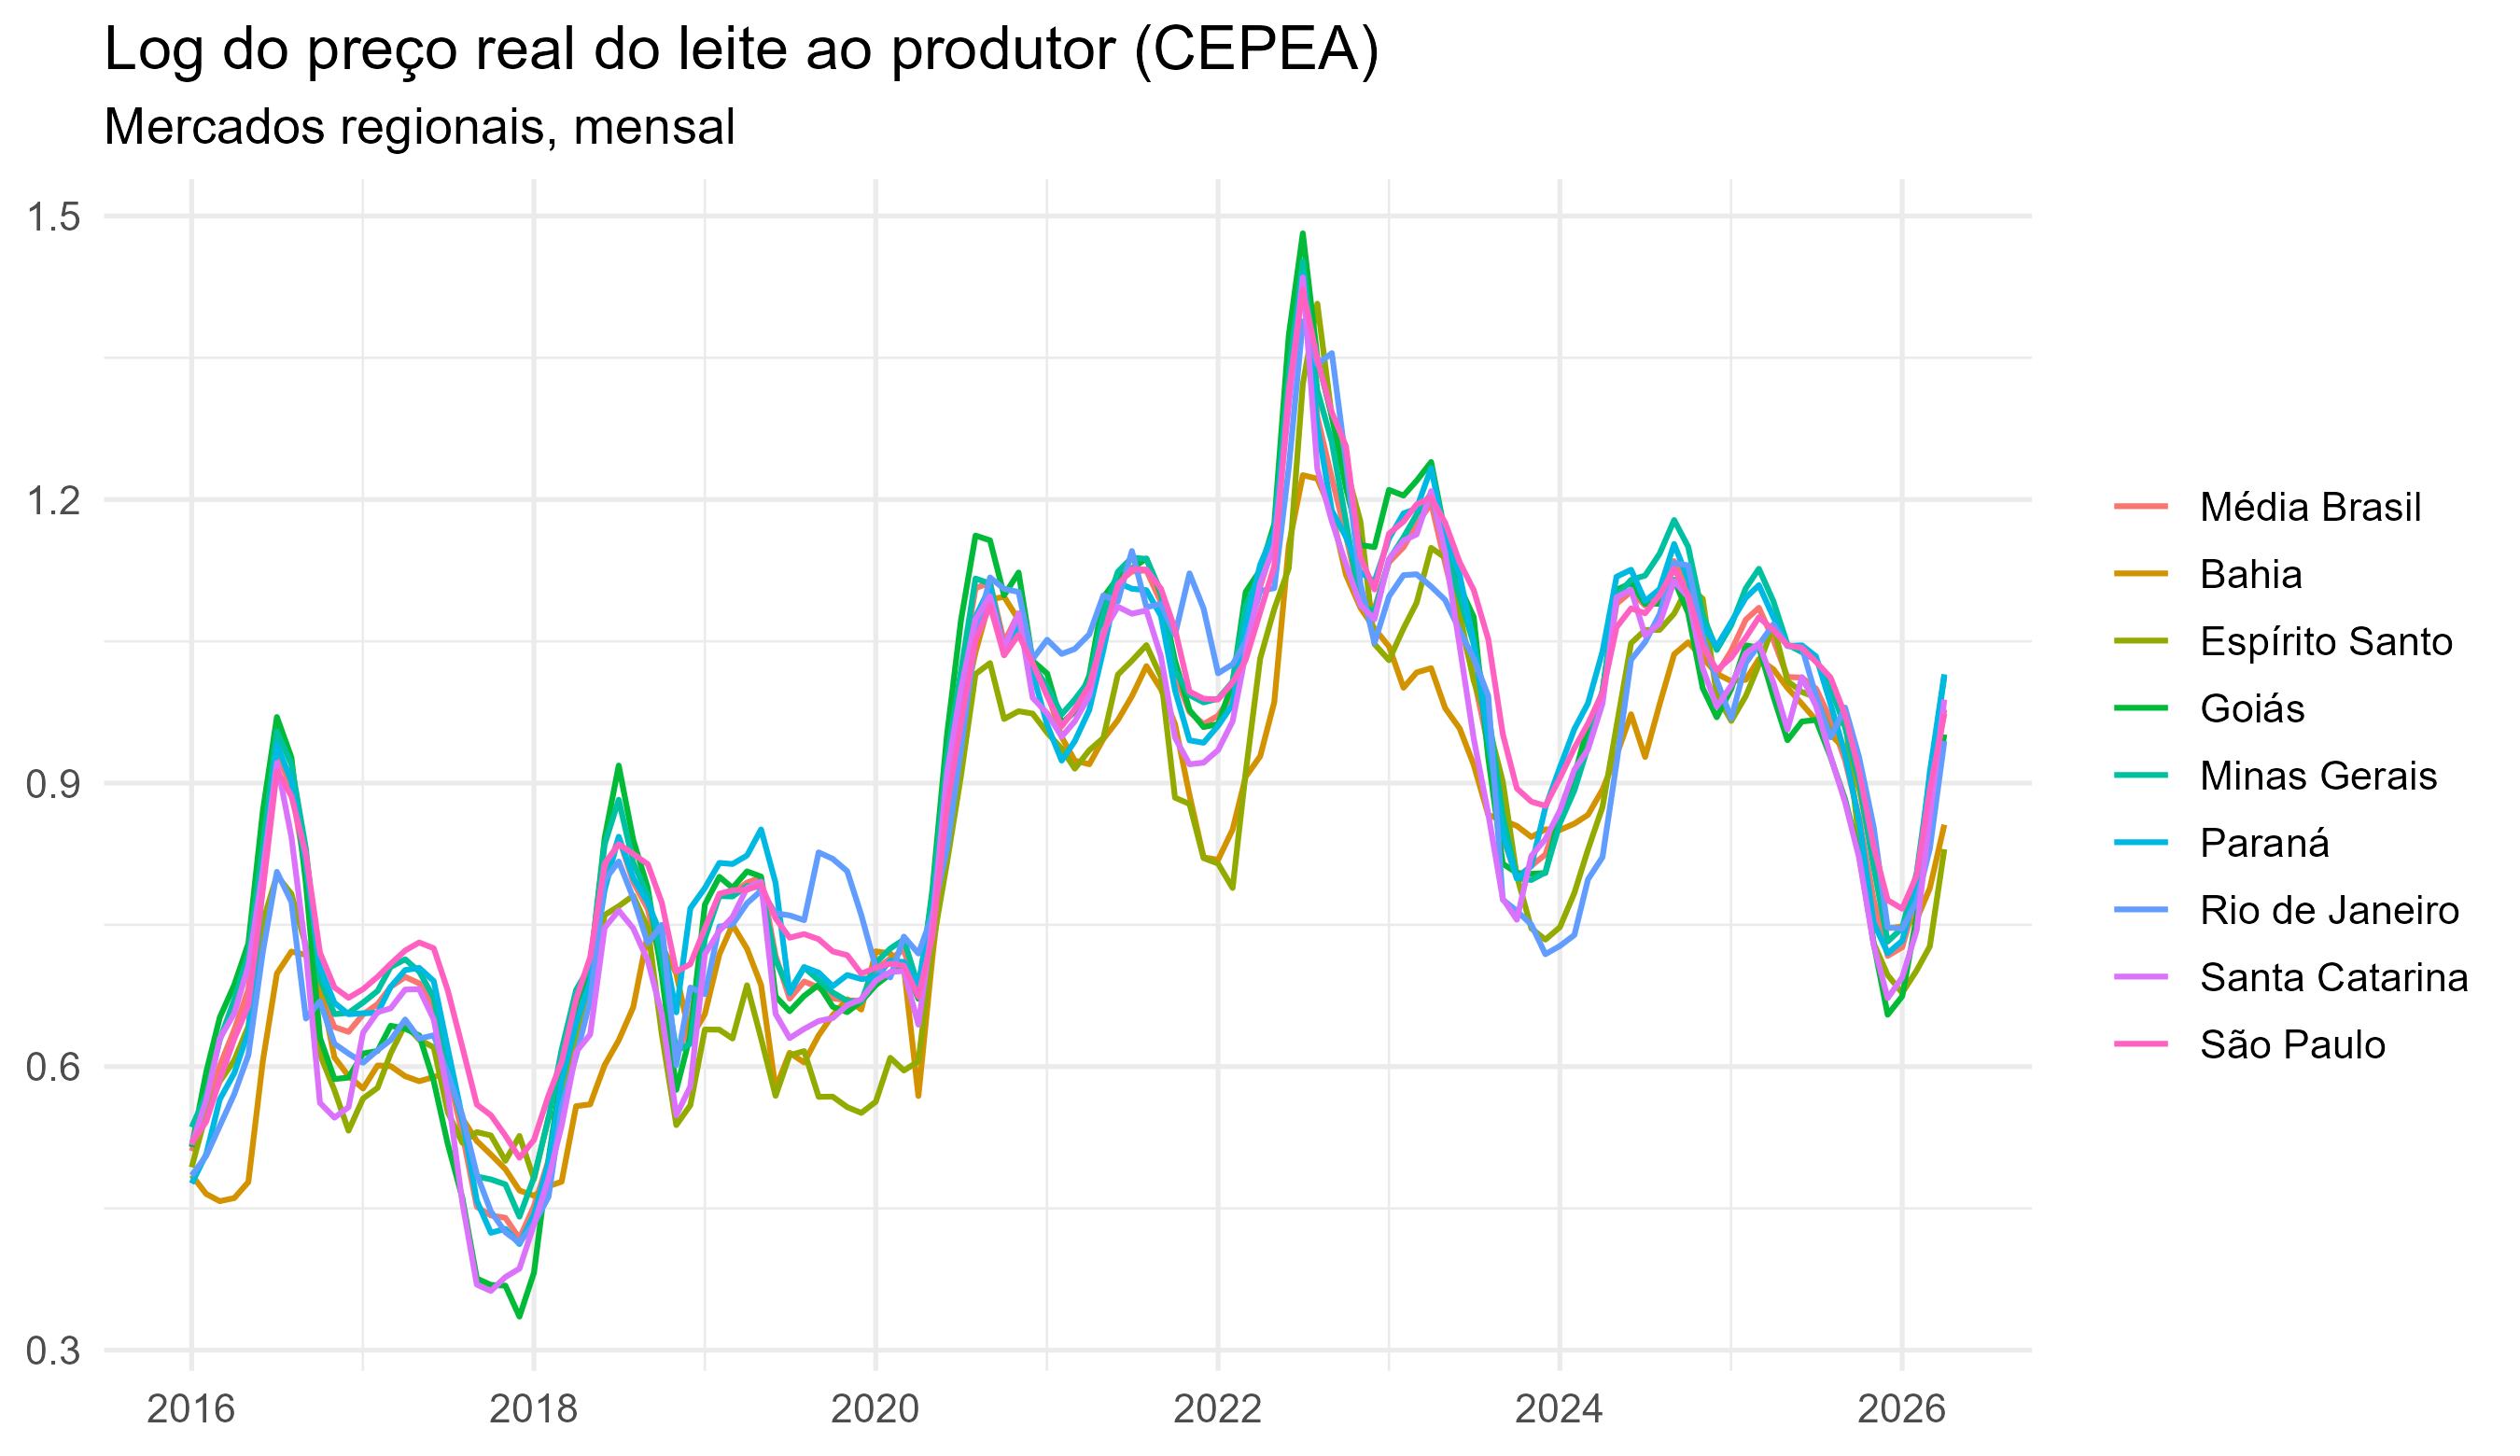
\includegraphics[width=0.82\textwidth]{fig01_series.png}
  \caption{Evolução do log do preço real do leite por região.}
  \label{fig:series}
\end{figure}

\begin{figure}[H]\centering
  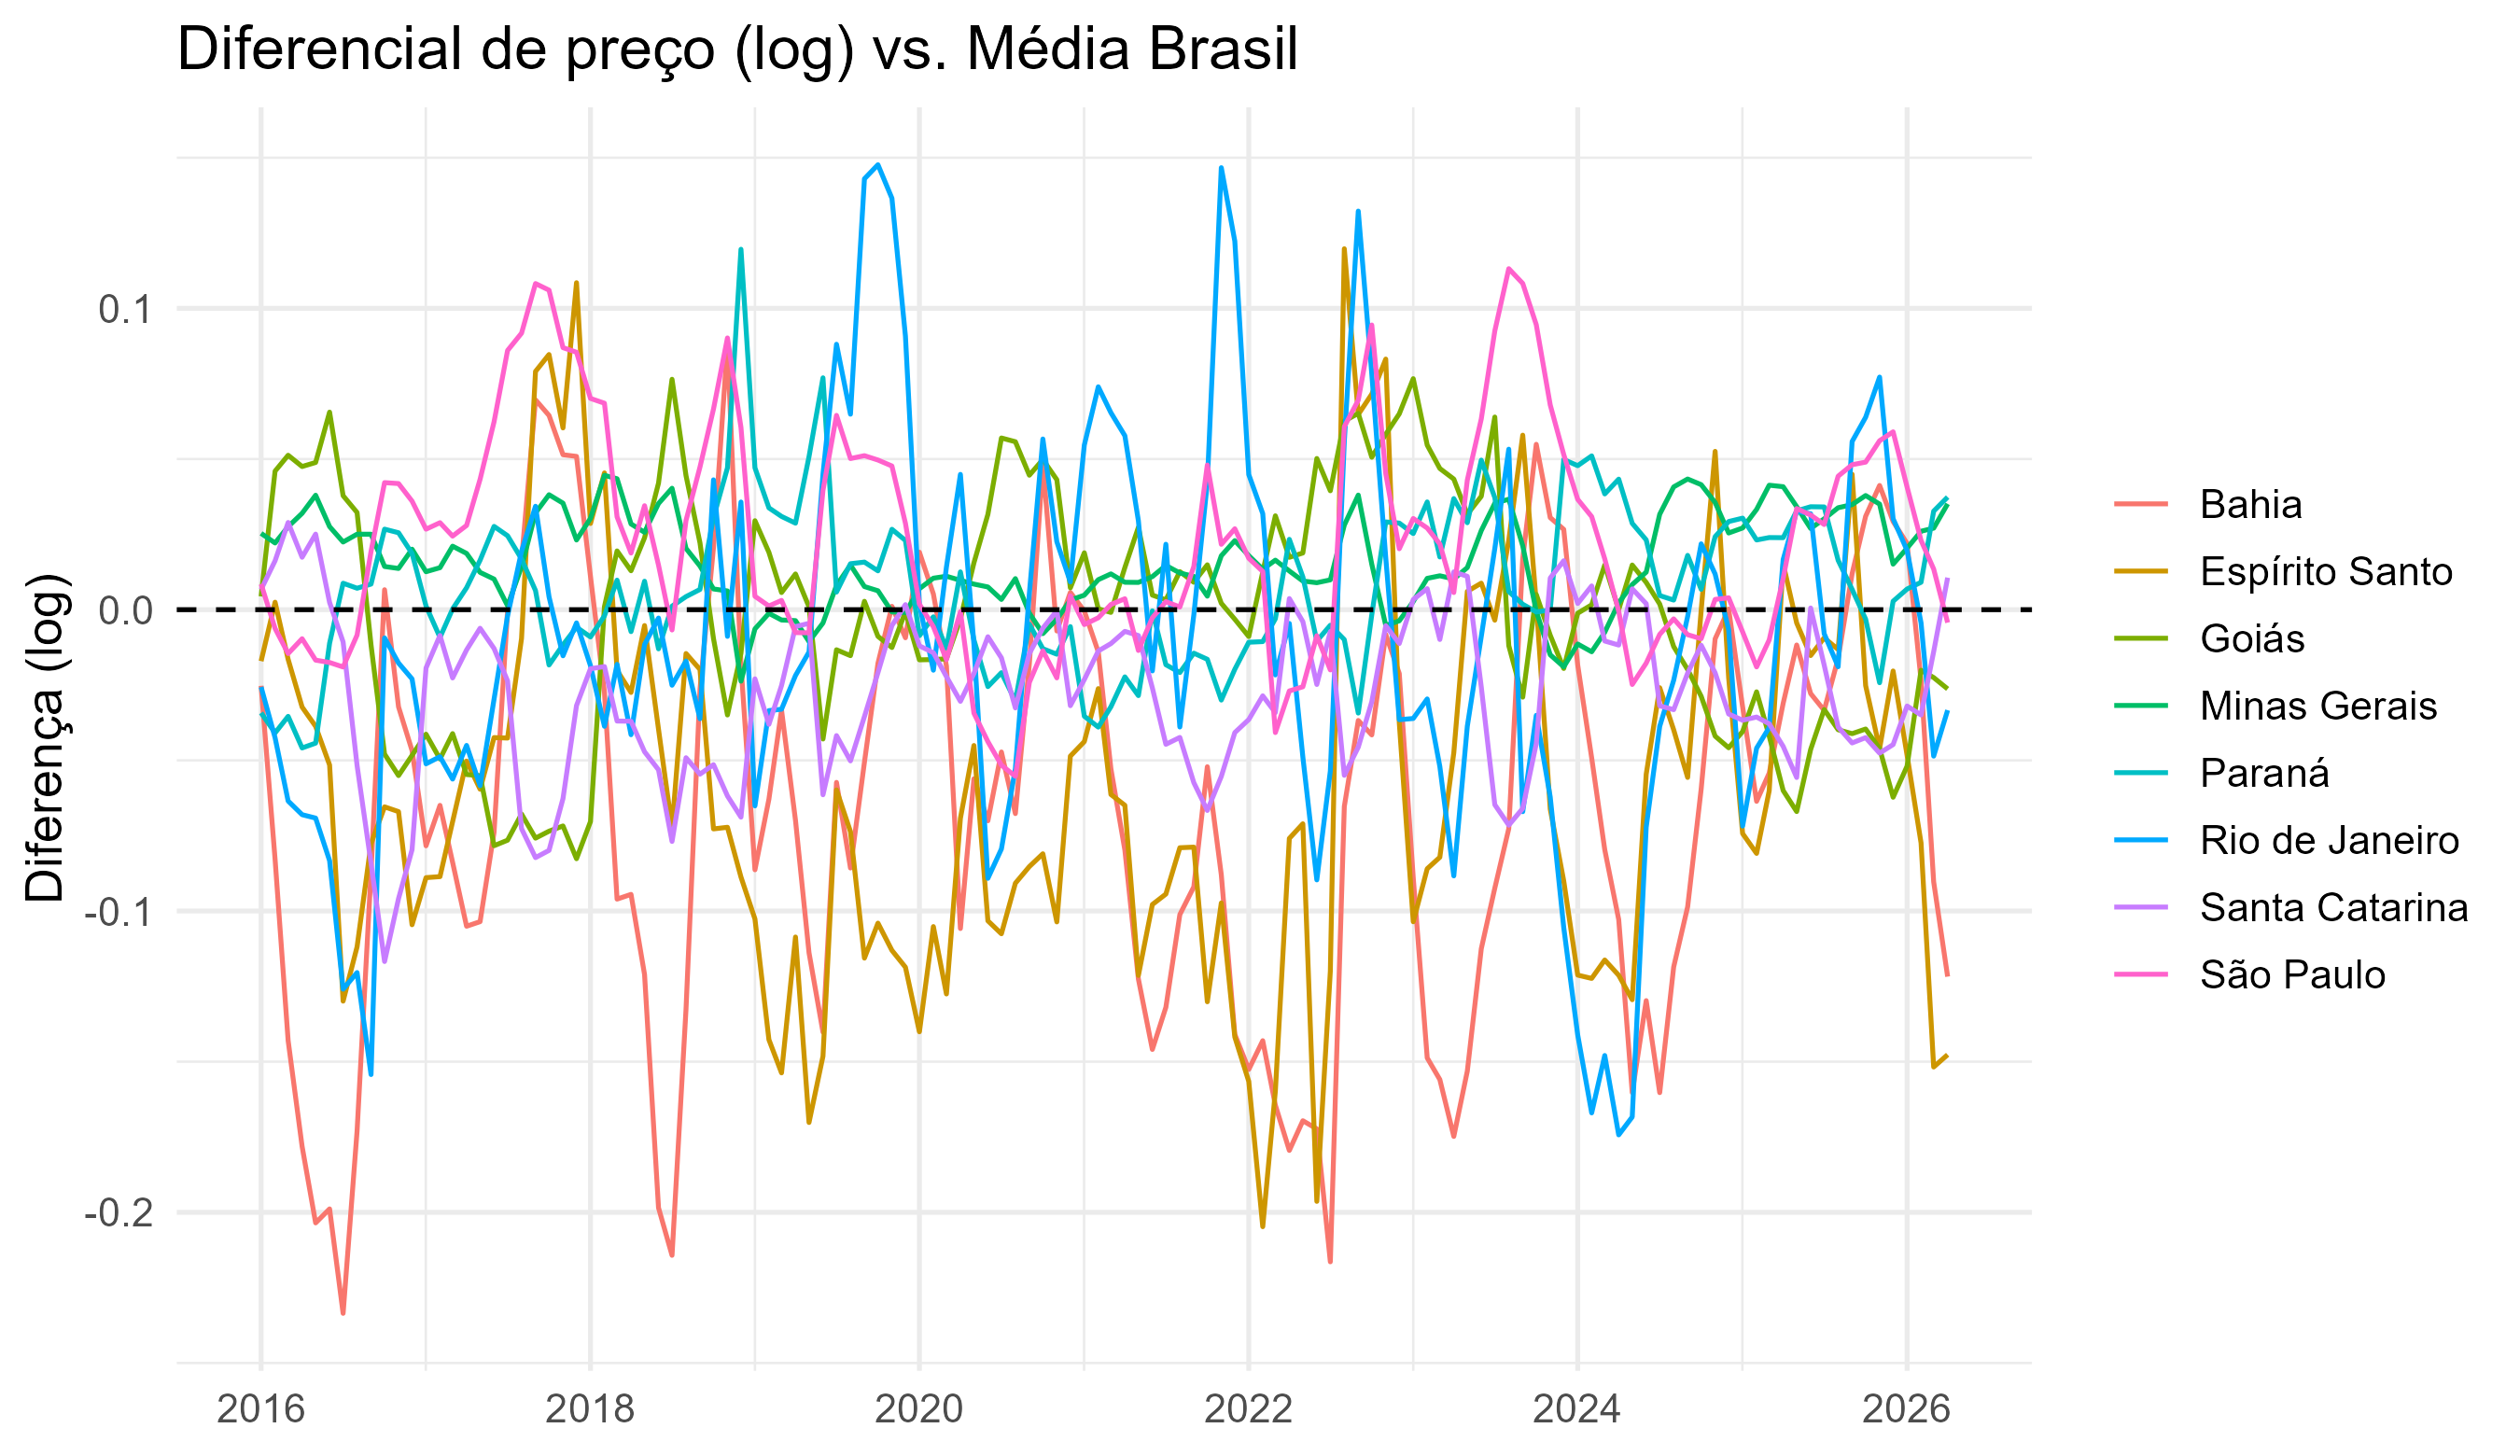
\includegraphics[width=0.82\textwidth]{fig02_spreads.png}
  \caption{Diferencial de preço (log) de cada estado em relação à Média Brasil.
  A oscilação em torno de zero sugere relação de equilíbrio de longo prazo.}
  \label{fig:spreads}
\end{figure}

\begin{figure}[H]\centering
  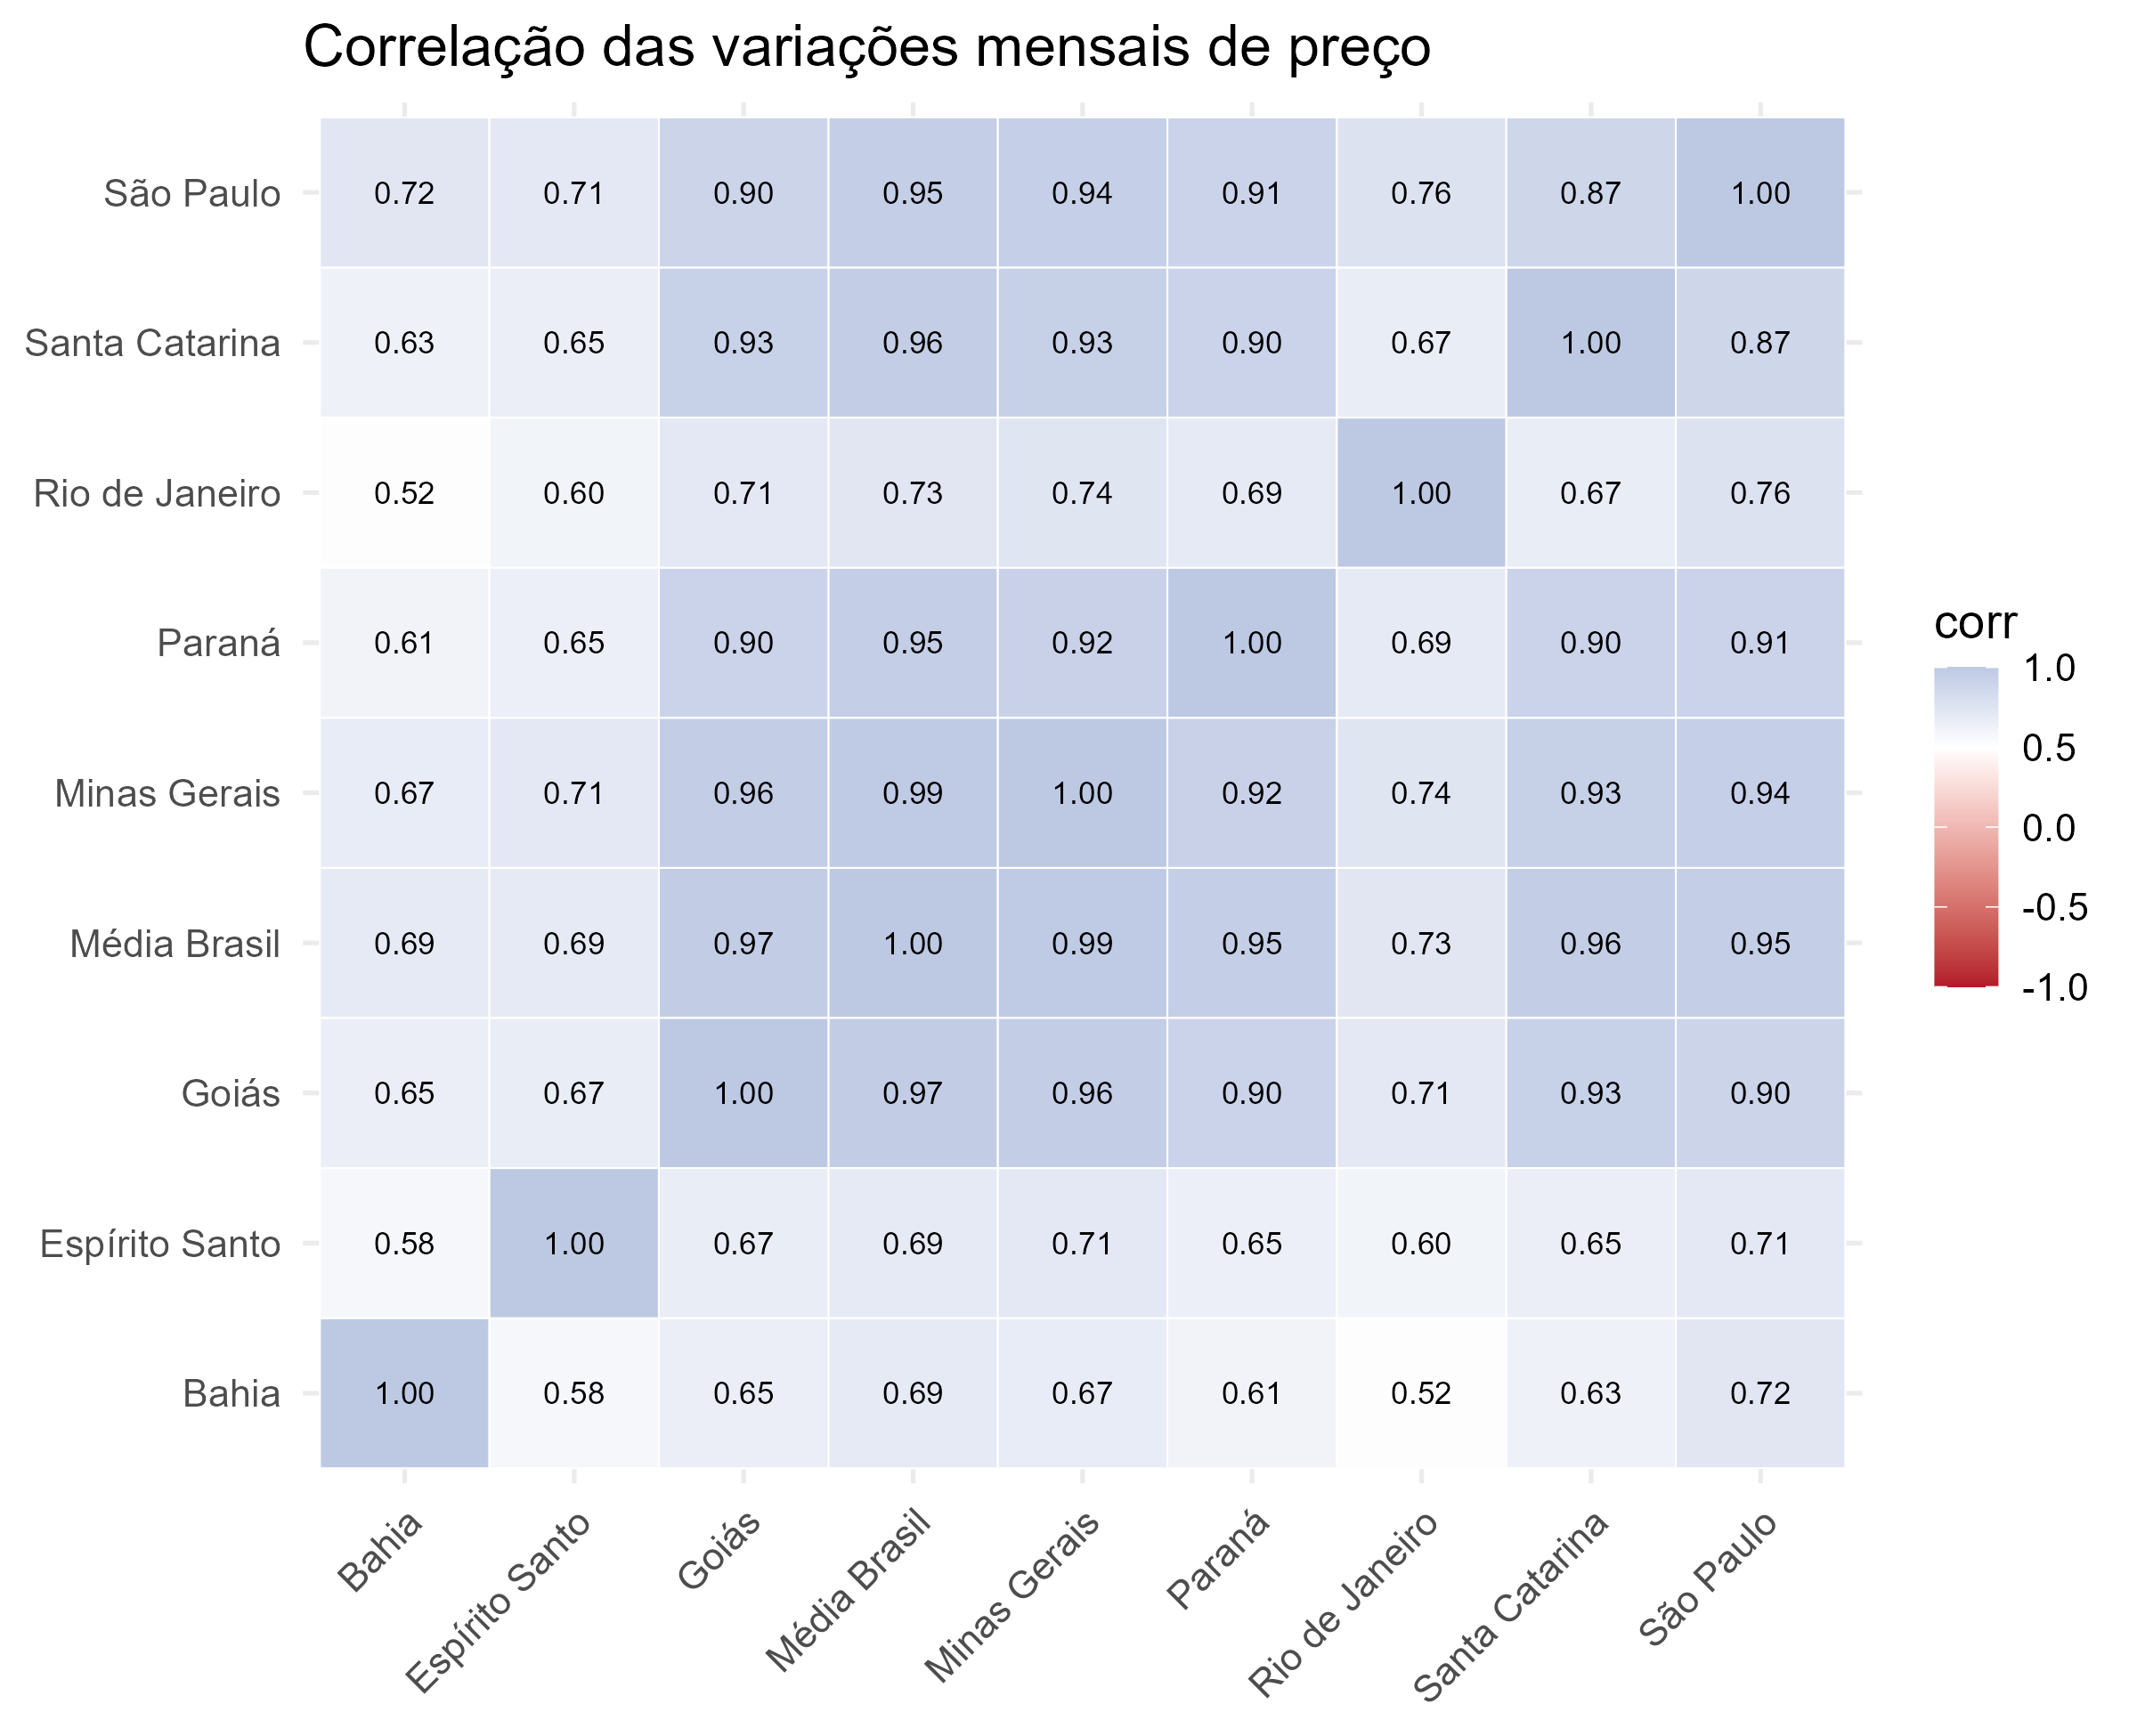
\includegraphics[width=0.7\textwidth]{fig03_corr_heatmap.png}
  \caption{Correlação das variações mensais de preço entre as regiões.}
  \label{fig:corr}
\end{figure}

% =====================================================================
\section{Estratégia empírica}
A sequência metodológica e as hipóteses de cada teste estão resumidas no
Quadro~\ref{quad:metodos}. Em termos práticos: primeiro verifica-se a ordem de
integração das séries; confirmando-se que são $I(1)$, testa-se a cointegração; havendo
cointegração, estima-se a dinâmica de curto prazo (ECM) e suas assimetrias; por fim,
modelos de limiar (TVECM) e o VAR fornecem, respectivamente, a banda de não-arbitragem e
a propagação de choques.

\begin{quadro}[!h]
\centering
\caption{\label{quad:metodos}Métodos, hipóteses e interpretação.}
\centering
\fontsize{9}{11}\selectfont
\begin{tabular}[t]{>{\raggedright\arraybackslash}p{3.4cm}>{\raggedright\arraybackslash}p{5.6cm}>{\raggedright\arraybackslash}p{6cm}}
\toprule
\textbf{Método} & \textbf{Hipótese nula ($H_0$)} & \textbf{Rejeitar $H_0$ indica}\\
\midrule
\cellcolor{gray!10}{ADF / Phillips-Perron} & \cellcolor{gray!10}{série tem raiz unitária} & \cellcolor{gray!10}{série estacionária}\\
KPSS & série é estacionária & série não estacionária\\
\cellcolor{gray!10}{Johansen (traço)} & \cellcolor{gray!10}{posto de cointegração $=r$} & \cellcolor{gray!10}{há relação(ões) de longo prazo}\\
Phillips-Ouliaris & não há cointegração & mercados cointegrados\\
\cellcolor{gray!10}{ECM assimétrico (Wald)} & \cellcolor{gray!10}{$\alpha^{+}=\alpha^{-}$ (simétrico)} & \cellcolor{gray!10}{transmissão assimétrica}\\
M-TAR (Enders-Siklos) & $\rho^{+}=\rho^{-}$ (simétrico) & assimetria no ajuste ao limiar\\
\cellcolor{gray!10}{Hansen-Seo} & \cellcolor{gray!10}{VECM linear} & \cellcolor{gray!10}{há efeito de limiar (TVECM)}\\
Granger & $X$ não antecede $Y$ & $X$ ajuda a prever $Y$\\
\bottomrule
\end{tabular}
\end{quadro}


% =====================================================================
\section{Resultados}

\subsection{Ordem de integração}
A Tabela~\ref{tab:raiz} reporta os testes de raiz unitária. Em nível, a maioria das
séries não rejeita fortemente a hipótese de raiz unitária pelos critérios conjuntos; em
primeira diferença, o ADF rejeita amplamente a raiz unitária. Conclui-se que os preços
são integrados de ordem 1, $I(1)$ --- condição necessária para a cointegração.

\begin{table}[!h]
\centering
\caption{\label{tab:raiz}Testes de raiz unitária (níveis em log).}
\centering
\fontsize{10}{12}\selectfont
\begin{tabular}[t]{lrrrr}
\toprule
\textbf{Região} & \textbf{ADF nível} & \textbf{ADF 1\textsuperscript{a} dif.} & \textbf{PP nível} & \textbf{KPSS nível}\\
\midrule
\cellcolor{gray!10}{Média Brasil} & \cellcolor{gray!10}{-3,968} & \cellcolor{gray!10}{-6,378} & \cellcolor{gray!10}{-2,746} & \cellcolor{gray!10}{0,276}\\
Bahia & -3,290 & -5,913 & -2,398 & 0,293\\
\cellcolor{gray!10}{Espírito Santo} & \cellcolor{gray!10}{-3,506} & \cellcolor{gray!10}{-5,994} & \cellcolor{gray!10}{-2,651} & \cellcolor{gray!10}{0,227}\\
Goiás & -3,798 & -6,694 & -2,686 & 0,292\\
\cellcolor{gray!10}{Minas Gerais} & \cellcolor{gray!10}{-4,116} & \cellcolor{gray!10}{-6,385} & \cellcolor{gray!10}{-2,833} & \cellcolor{gray!10}{0,253}\\
Paraná & -4,067 & -6,207 & -2,937 & 0,257\\
\cellcolor{gray!10}{Rio de Janeiro} & \cellcolor{gray!10}{-2,837} & \cellcolor{gray!10}{-5,425} & \cellcolor{gray!10}{-2,494} & \cellcolor{gray!10}{0,331}\\
Santa Catarina & -3,759 & -6,407 & -2,828 & 0,278\\
\cellcolor{gray!10}{São Paulo} & \cellcolor{gray!10}{-4,062} & \cellcolor{gray!10}{-6,223} & \cellcolor{gray!10}{-2,639} & \cellcolor{gray!10}{0,290}\\
\bottomrule
\end{tabular}
\end{table}


\noindent{\footnotesize\textit{Nota:} valores críticos a 5\%: ADF (com tendência)
$\approx -3{,}43$; KPSS $\approx 0{,}146$. ADF/PP: rejeitar $H_0$ (raiz unitária) se a
estatística for inferior ao crítico; KPSS: rejeitar estacionariedade se a estatística
superar o crítico.\par}

\subsection{Cointegração e correção de erro}
O teste de Johansen sobre o sistema completo indica a existência de relações de
cointegração entre as nove séries. Na análise par a par (Tabela~\ref{tab:par}), o teste
de Phillips-Ouliaris confirma cointegração com a Média Brasil para a maioria dos estados.
As elasticidades de longo prazo ($\beta$) situam-se próximas de 1 (0,87 a 1,09),
compatíveis com a Lei do Preço Único.

O termo de correção de erro ($\alpha$) é negativo e significativo em todos os casos,
indicando convergência ao equilíbrio, com velocidades de ajuste de $\approx 15\%$
(Goiás) a $46\%$ ao mês (Santa Catarina). A comparação entre $\alpha^{+}$ e $\alpha^{-}$
e o teste M-TAR, em geral, não rejeita a simetria: a transmissão de altas e de baixas
ocorre a velocidades semelhantes na maioria dos estados.

\begin{table}[!h]
\centering
\caption{\label{tab:par}Transmissão de preços, par a par (estado vs.\ Média Brasil).}
\centering
\resizebox{\ifdim\width>\linewidth\linewidth\else\width\fi}{!}{
\begin{tabular}[t]{lcccccccccc}
\toprule
\textbf{Estado} & \textbf{Coint. (P-O)} & \textbf{$\beta_{LP}$} & \textbf{$\alpha$} & \textbf{$p(\alpha)$} & \textbf{$\alpha^{+}$} & \textbf{$\alpha^{-}$} & \textbf{Assim. ECM} & \textbf{Assim. M-TAR} & \textbf{Granger ref$\to$est} & \textbf{Granger est$\to$ref}\\
\midrule
\cellcolor{gray!10}{Bahia} & \cellcolor{gray!10}{Sim} & \cellcolor{gray!10}{0,874} & \cellcolor{gray!10}{-0,221} & \cellcolor{gray!10}{$<$0,001} & \cellcolor{gray!10}{-0,231} & \cellcolor{gray!10}{-0,213} & \cellcolor{gray!10}{0,888} & \cellcolor{gray!10}{0,872} & \cellcolor{gray!10}{$<$0,001} & \cellcolor{gray!10}{0,006}\\
Espírito Santo & Sim & 0,952 & -0,211 & 0,001 & -0,172 & -0,261 & 0,628 & 0,063 & $<$0,001 & 0,644\\
\cellcolor{gray!10}{Goiás} & \cellcolor{gray!10}{Não} & \cellcolor{gray!10}{1,088} & \cellcolor{gray!10}{-0,150} & \cellcolor{gray!10}{0,004} & \cellcolor{gray!10}{-0,226} & \cellcolor{gray!10}{-0,077} & \cellcolor{gray!10}{0,285} & \cellcolor{gray!10}{0,571} & \cellcolor{gray!10}{0,638} & \cellcolor{gray!10}{0,006}\\
Minas Gerais & Sim & 0,997 & -0,162 & 0,003 & -0,169 & -0,154 & 0,934 & 0,267 & 0,255 & 0,613\\
\cellcolor{gray!10}{Paraná} & \cellcolor{gray!10}{Sim} & \cellcolor{gray!10}{1,001} & \cellcolor{gray!10}{-0,278} & \cellcolor{gray!10}{$<$0,001} & \cellcolor{gray!10}{-0,434} & \cellcolor{gray!10}{-0,098} & \cellcolor{gray!10}{0,085} & \cellcolor{gray!10}{0,650} & \cellcolor{gray!10}{0,003} & \cellcolor{gray!10}{0,133}\\
Rio de Janeiro & Sim & 0,983 & -0,244 & $<$0,001 & -0,332 & -0,156 & 0,283 & 0,717 & $<$0,001 & 0,445\\
\cellcolor{gray!10}{Santa Catarina} & \cellcolor{gray!10}{Sim} & \cellcolor{gray!10}{1,025} & \cellcolor{gray!10}{-0,461} & \cellcolor{gray!10}{$<$0,001} & \cellcolor{gray!10}{-0,451} & \cellcolor{gray!10}{-0,470} & \cellcolor{gray!10}{0,914} & \cellcolor{gray!10}{0,273} & \cellcolor{gray!10}{0,001} & \cellcolor{gray!10}{0,041}\\
São Paulo & Não & 0,928 & -0,201 & $<$0,001 & -0,215 & -0,181 & 0,772 & 0,413 & 0,017 & 0,040\\
\bottomrule
\end{tabular}}
\end{table}


\noindent{\footnotesize\textit{Nota:} $\beta_{LP}$ = elasticidade de longo prazo;
$\alpha$ = velocidade de ajuste mensal; $\alpha^{+}/\alpha^{-}$ = ajuste a desvios
positivos/negativos; as colunas de assimetria e Granger reportam valores-$p$;
Coint.\ (P-O) = cointegração pelo teste de Phillips-Ouliaris a 5\%.\par}

\subsection{Modelo com limiar (TVECM) e banda de não-arbitragem}
O TVECM permite que a velocidade de ajuste mude conforme o tamanho do desvio do
equilíbrio. A intuição econômica é a \emph{banda de não-arbitragem}: enquanto o desvio
for menor que os custos de transação (regime interno), não compensa arbitrar e o ajuste é
fraco; quando o desvio ultrapassa o limiar (regime externo), a arbitragem espacial age e
o preço retorna rapidamente ao equilíbrio. A Tabela~\ref{tab:tvecm} traz o limiar
estimado, as velocidades de ajuste por regime e o teste de Hansen-Seo.

Para vários pares, o ajuste é nitidamente mais forte em um dos regimes, e o teste de
Hansen-Seo aponta efeito de limiar relevante ($p \le 0{,}05$, p.ex.\ Minas Gerais e São
Paulo), corroborando a hipótese de custos de transação na integração espacial. A
Figura~\ref{fig:tvecm} ilustra o mecanismo: a inclinação mais acentuada à esquerda do
limiar evidencia o regime de ajuste rápido.

\begin{table}[!h]
\centering
\caption{\label{tab:tvecm}VECM com limiar (TVECM): estado vs.\ Média Brasil. Regime~1 = desvios abaixo do limiar; regime~2 = acima.}
\centering
\fontsize{9}{11}\selectfont
\begin{tabular}[t]{lrrrrrrr}
\toprule
\textbf{Estado} & \textbf{Limiar} & \textbf{$\beta_{LP}$} & \textbf{$\alpha$ reg.\ 1} & \textbf{$\alpha$ reg.\ 2} & \textbf{$n_1$} & \textbf{$n_2$} & \textbf{Hansen-Seo ($p$)}\\
\midrule
\cellcolor{gray!10}{Bahia} & \cellcolor{gray!10}{-0,0306} & \cellcolor{gray!10}{0,890} & \cellcolor{gray!10}{0,017} & \cellcolor{gray!10}{-0,000} & \cellcolor{gray!10}{23} & \cellcolor{gray!10}{99} & \cellcolor{gray!10}{0,090}\\
Espírito Santo & 0,0131 & 0,919 & -0,496 & -0,414 & 66 & 56 & 0,170\\
\cellcolor{gray!10}{Goiás} & \cellcolor{gray!10}{-0,0054} & \cellcolor{gray!10}{0,980} & \cellcolor{gray!10}{-0,438} & \cellcolor{gray!10}{-0,595} & \cellcolor{gray!10}{35} & \cellcolor{gray!10}{87} & \cellcolor{gray!10}{0,600}\\
Minas Gerais & -0,0150 & 1,018 & -6,192 & -0,315 & 20 & 102 & 0,050\\
\cellcolor{gray!10}{Paraná} & \cellcolor{gray!10}{0,0194} & \cellcolor{gray!10}{0,978} & \cellcolor{gray!10}{-0,663} & \cellcolor{gray!10}{0,104} & \cellcolor{gray!10}{47} & \cellcolor{gray!10}{75} & \cellcolor{gray!10}{0,420}\\
Rio de Janeiro & 0,0303 & 1,023 & -0,159 & -0,377 & 103 & 19 & 0,960\\
\cellcolor{gray!10}{Santa Catarina} & \cellcolor{gray!10}{0,0268} & \cellcolor{gray!10}{0,961} & \cellcolor{gray!10}{-0,500} & \cellcolor{gray!10}{-2,302} & \cellcolor{gray!10}{92} & \cellcolor{gray!10}{30} & \cellcolor{gray!10}{0,260}\\
São Paulo & 0,0149 & 0,981 & -1,938 & -0,206 & 34 & 88 & 0,050\\
\bottomrule
\end{tabular}
\end{table}


\noindent{\footnotesize\textit{Nota:} $\alpha$ reg.\ = velocidade de ajuste por regime;
$n_1,n_2$ = nº de observações em cada regime; Hansen-Seo = valor-$p$ do teste de efeito
de limiar (rejeitar $H_0$ linear se $p<0{,}05$). Coeficientes de regimes com poucas
observações devem ser lidos com cautela.\par}

\begin{figure}[H]\centering
  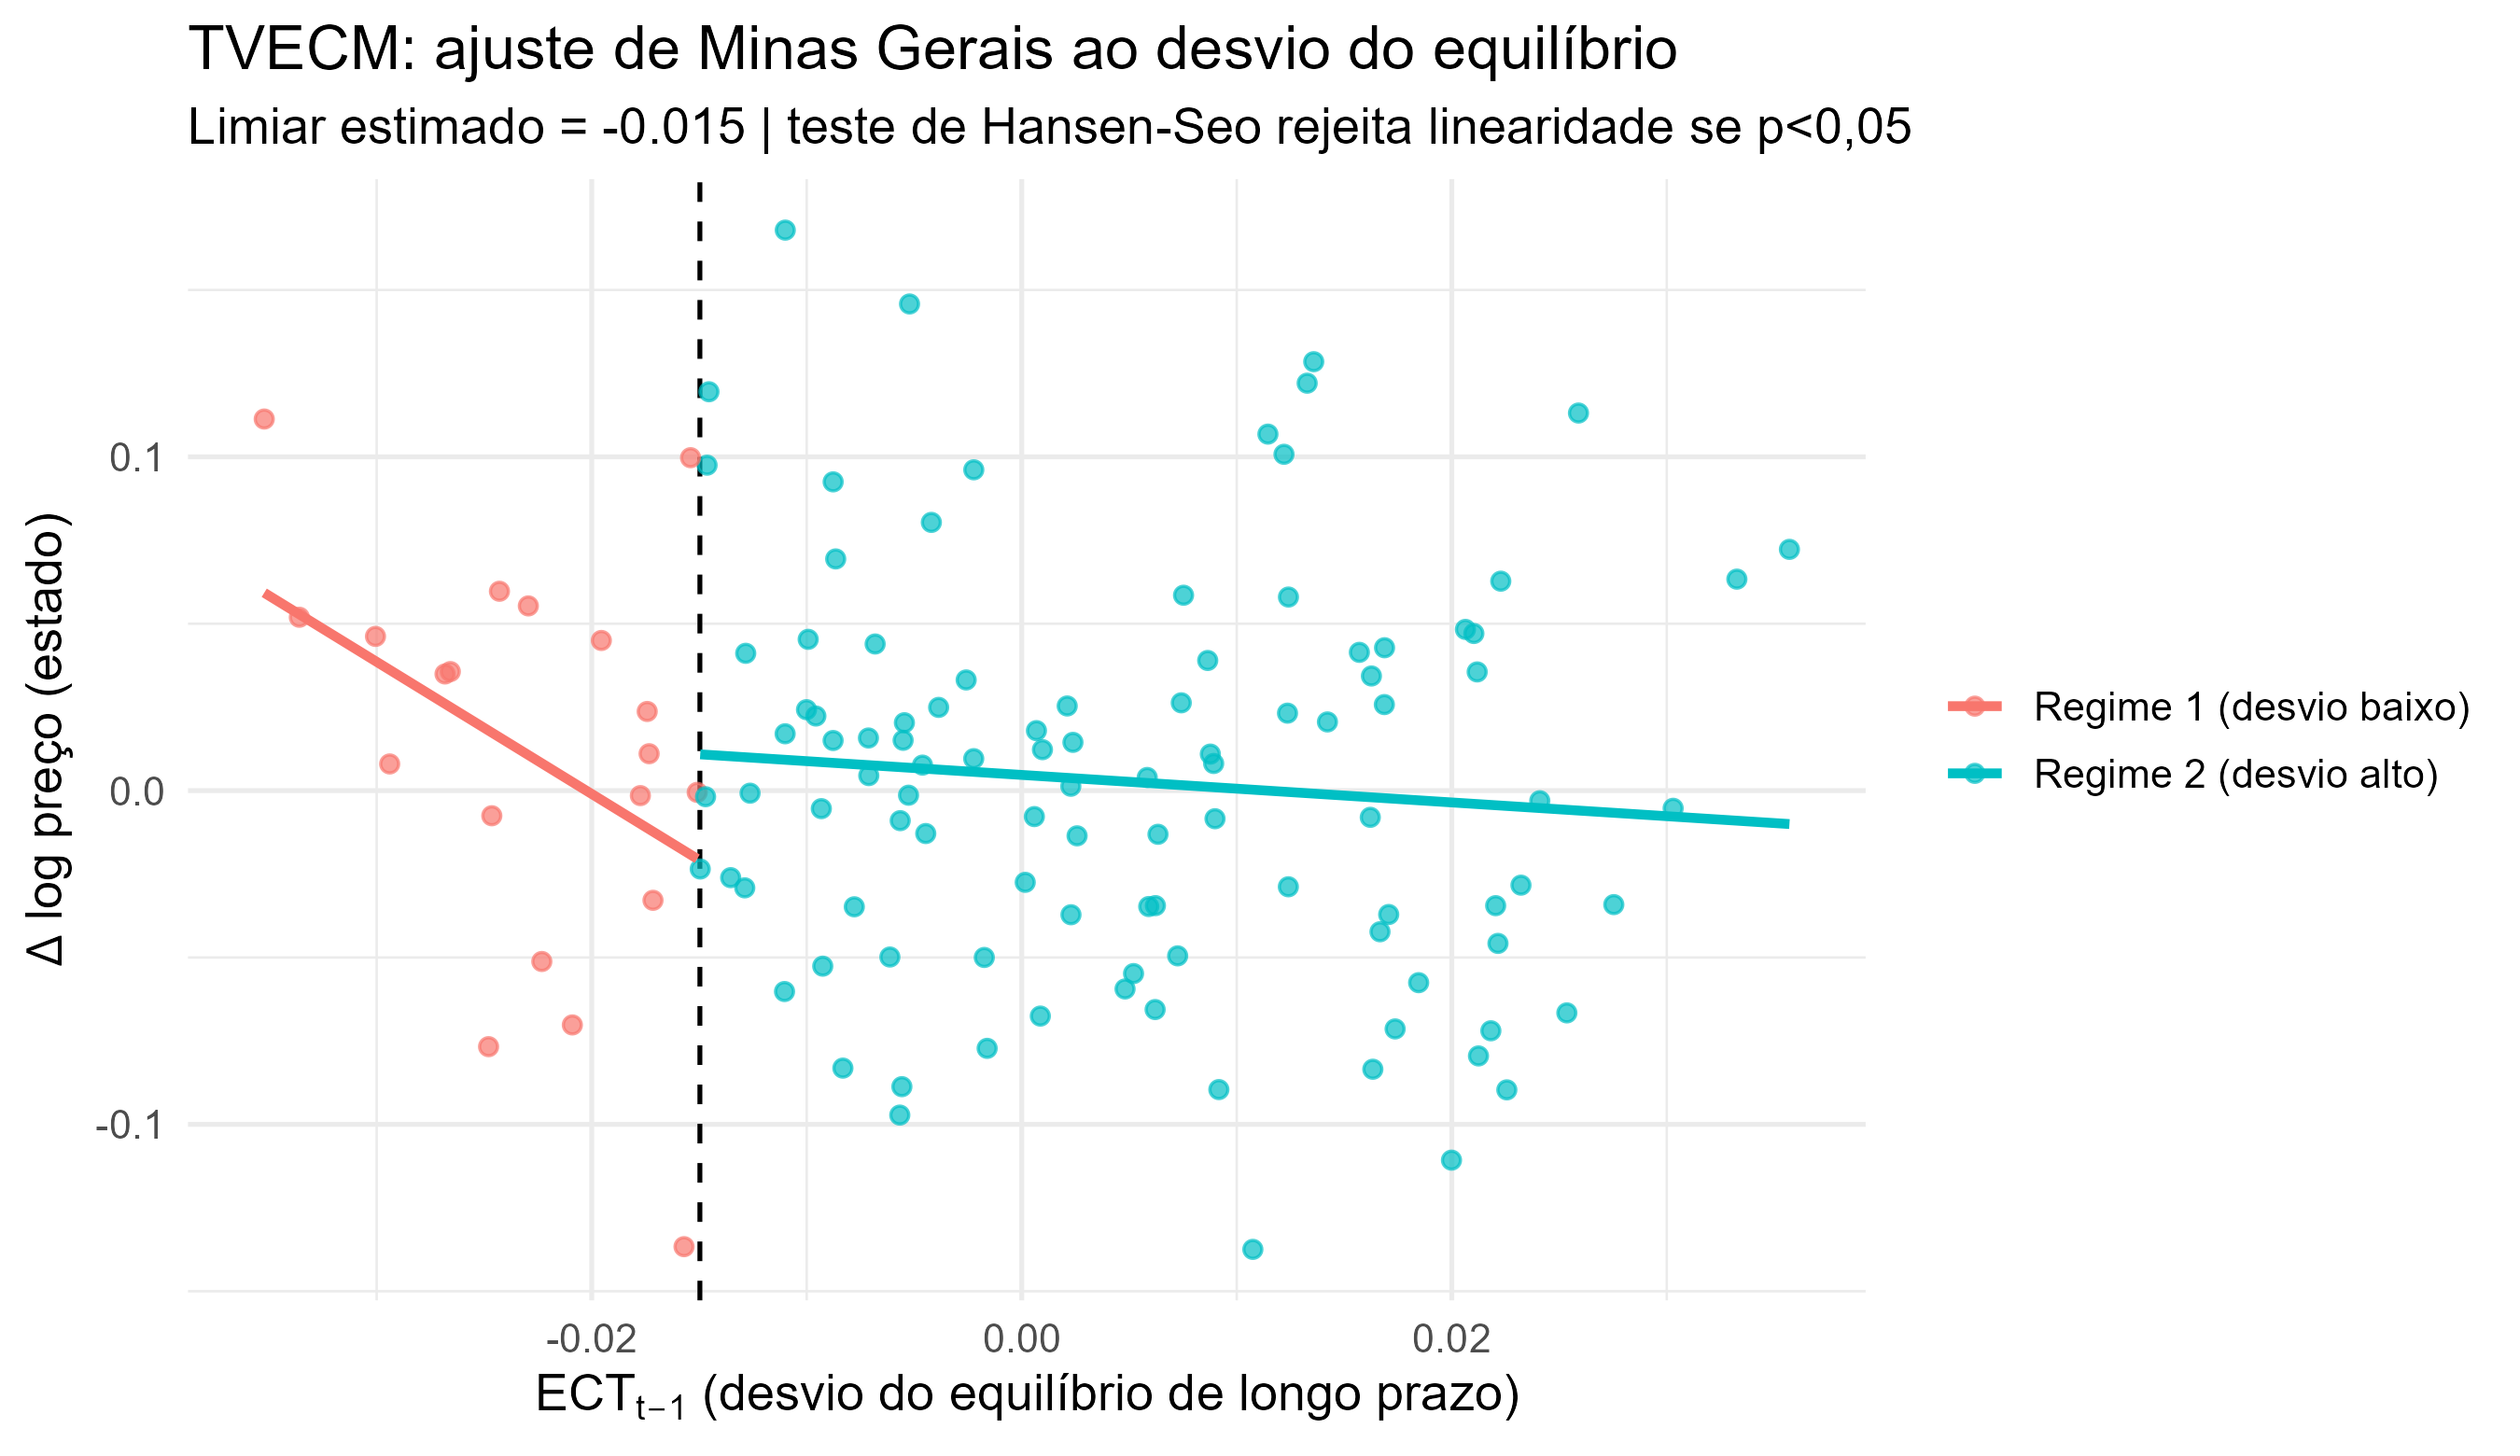
\includegraphics[width=0.82\textwidth]{fig04_tvecm_regimes.png}
  \caption{TVECM: ajuste do preço ao desvio do equilíbrio, por regime, com o limiar
  estimado (linha tracejada).}
  \label{fig:tvecm}
\end{figure}

\subsection{Causalidade de Granger}
A matriz de causalidade de Granger (Figura~\ref{fig:granger}) mostra a estrutura de
precedência temporal. A Média Brasil e estados de grande peso na produção (Minas Gerais,
São Paulo) antecedem sistematicamente os demais, sinal de liderança no descobrimento de
preços; alguns pares exibem causalidade bidirecional.

\begin{figure}[H]\centering
  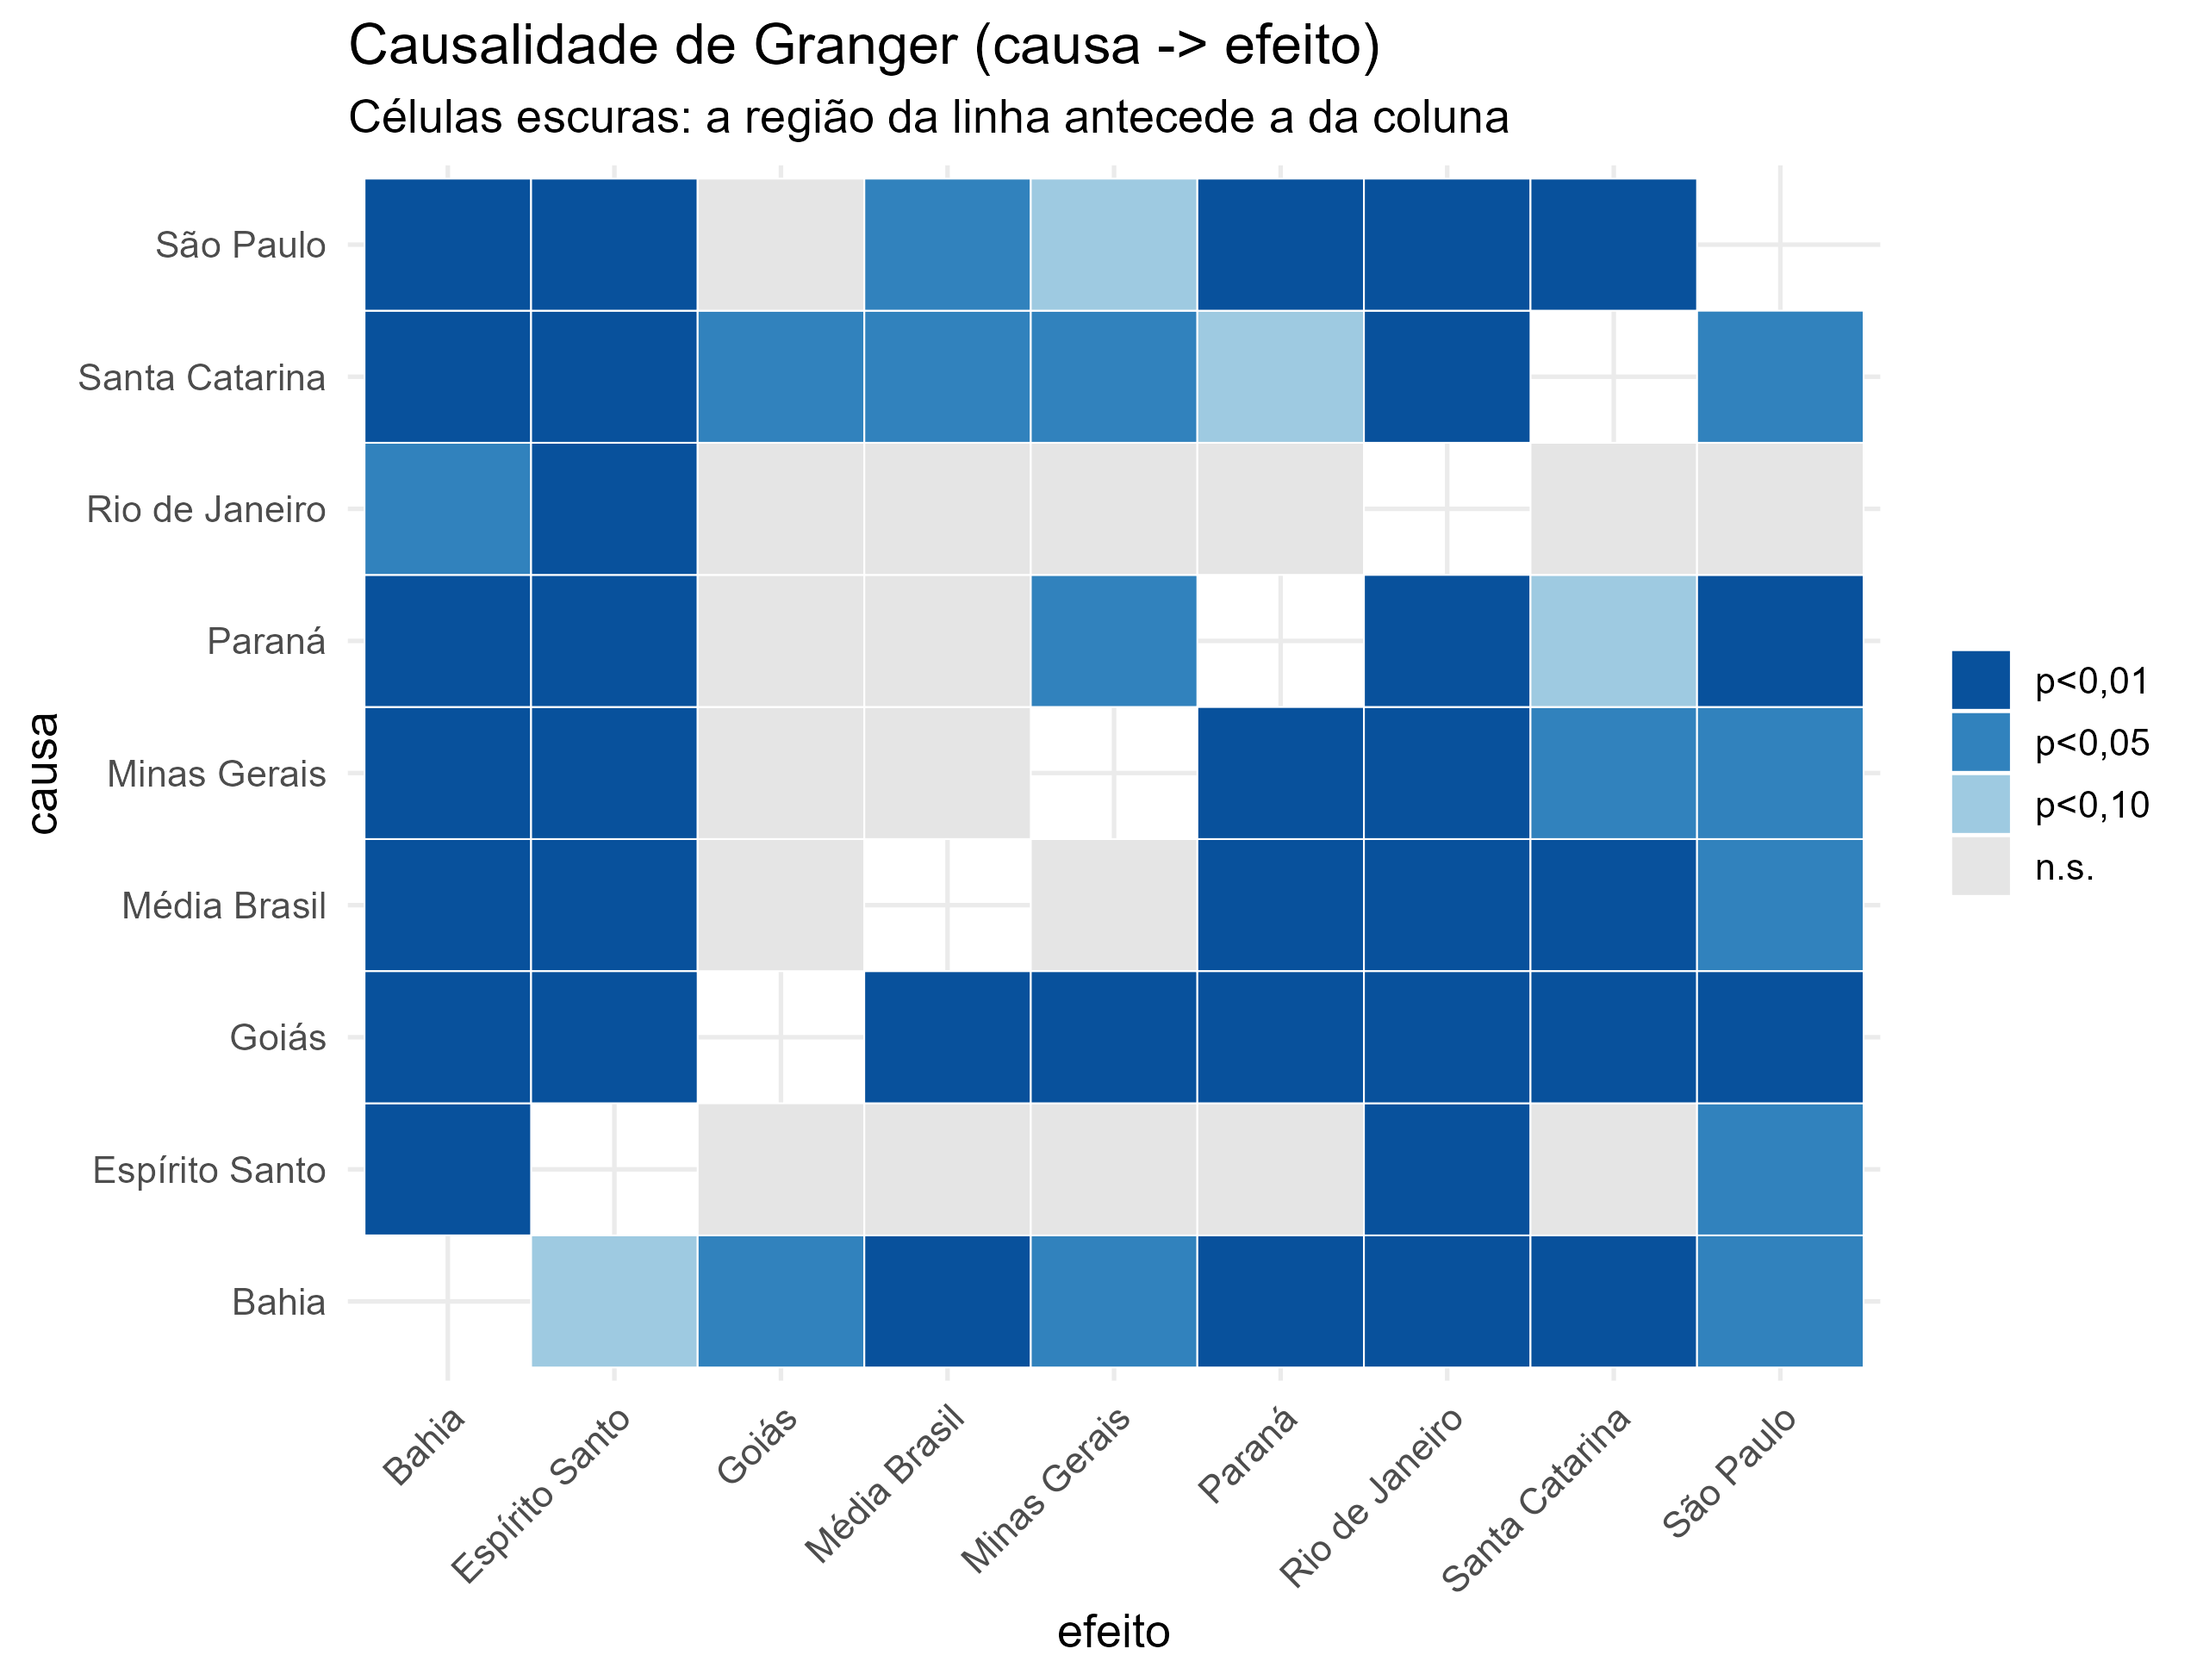
\includegraphics[width=0.75\textwidth]{fig05_granger_heatmap.png}
  \caption{Causalidade de Granger (causa $\to$ efeito). Células escuras indicam que a
  região da linha antecede a da coluna.}
  \label{fig:granger}
\end{figure}

\subsection{Impulso-resposta e decomposição da variância}
As funções de impulso-resposta (Figura~\ref{fig:irf}) mostram resposta positiva dos
estados a um choque na referência, dissipada em poucos meses. A decomposição da variância
a 12 meses (Figura~\ref{fig:fevd} e Tabela~\ref{tab:fevd}) indica que o preço de
referência explica parcela majoritária da variância dos estados mais integrados
(Paraná $\approx 66\%$, Santa Catarina $\approx 61\%$, Minas Gerais $\approx 60\%$).

\begin{figure}[H]\centering
  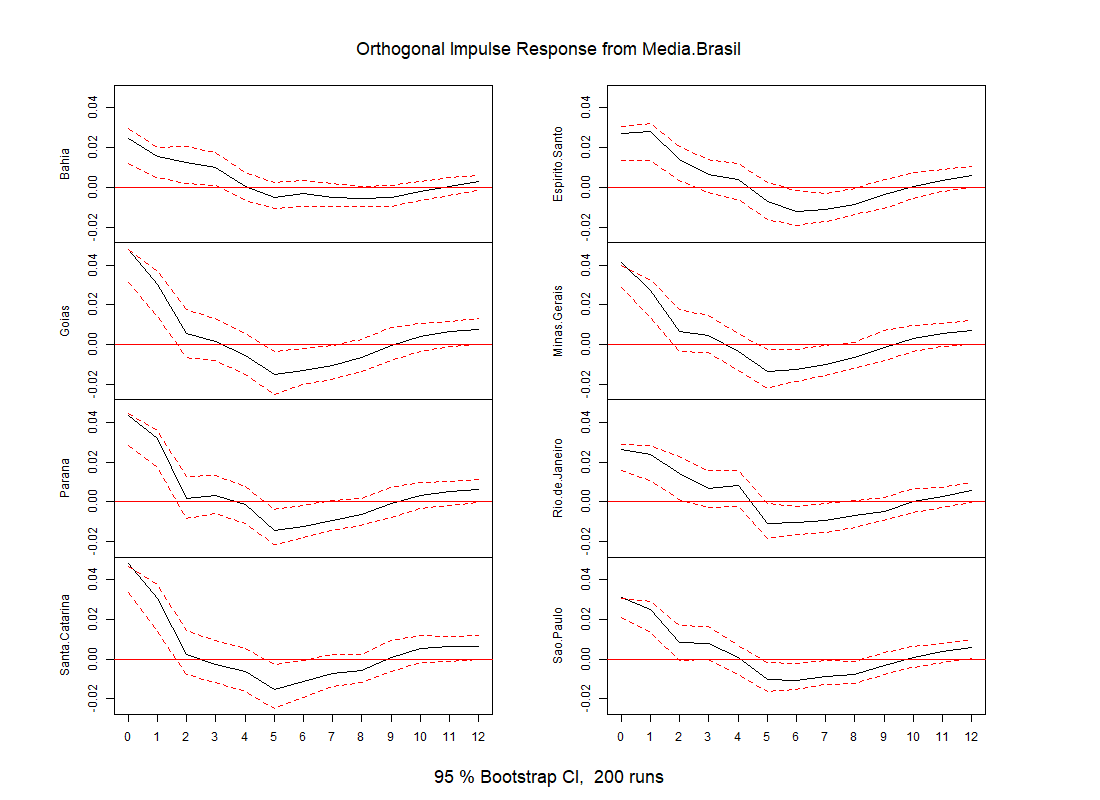
\includegraphics[width=0.85\textwidth]{fig06_irf.png}
  \caption{Funções de impulso-resposta: reação dos estados a um choque na Média Brasil
  (bandas de 95\% por bootstrap).}
  \label{fig:irf}
\end{figure}

\begin{figure}[H]\centering
  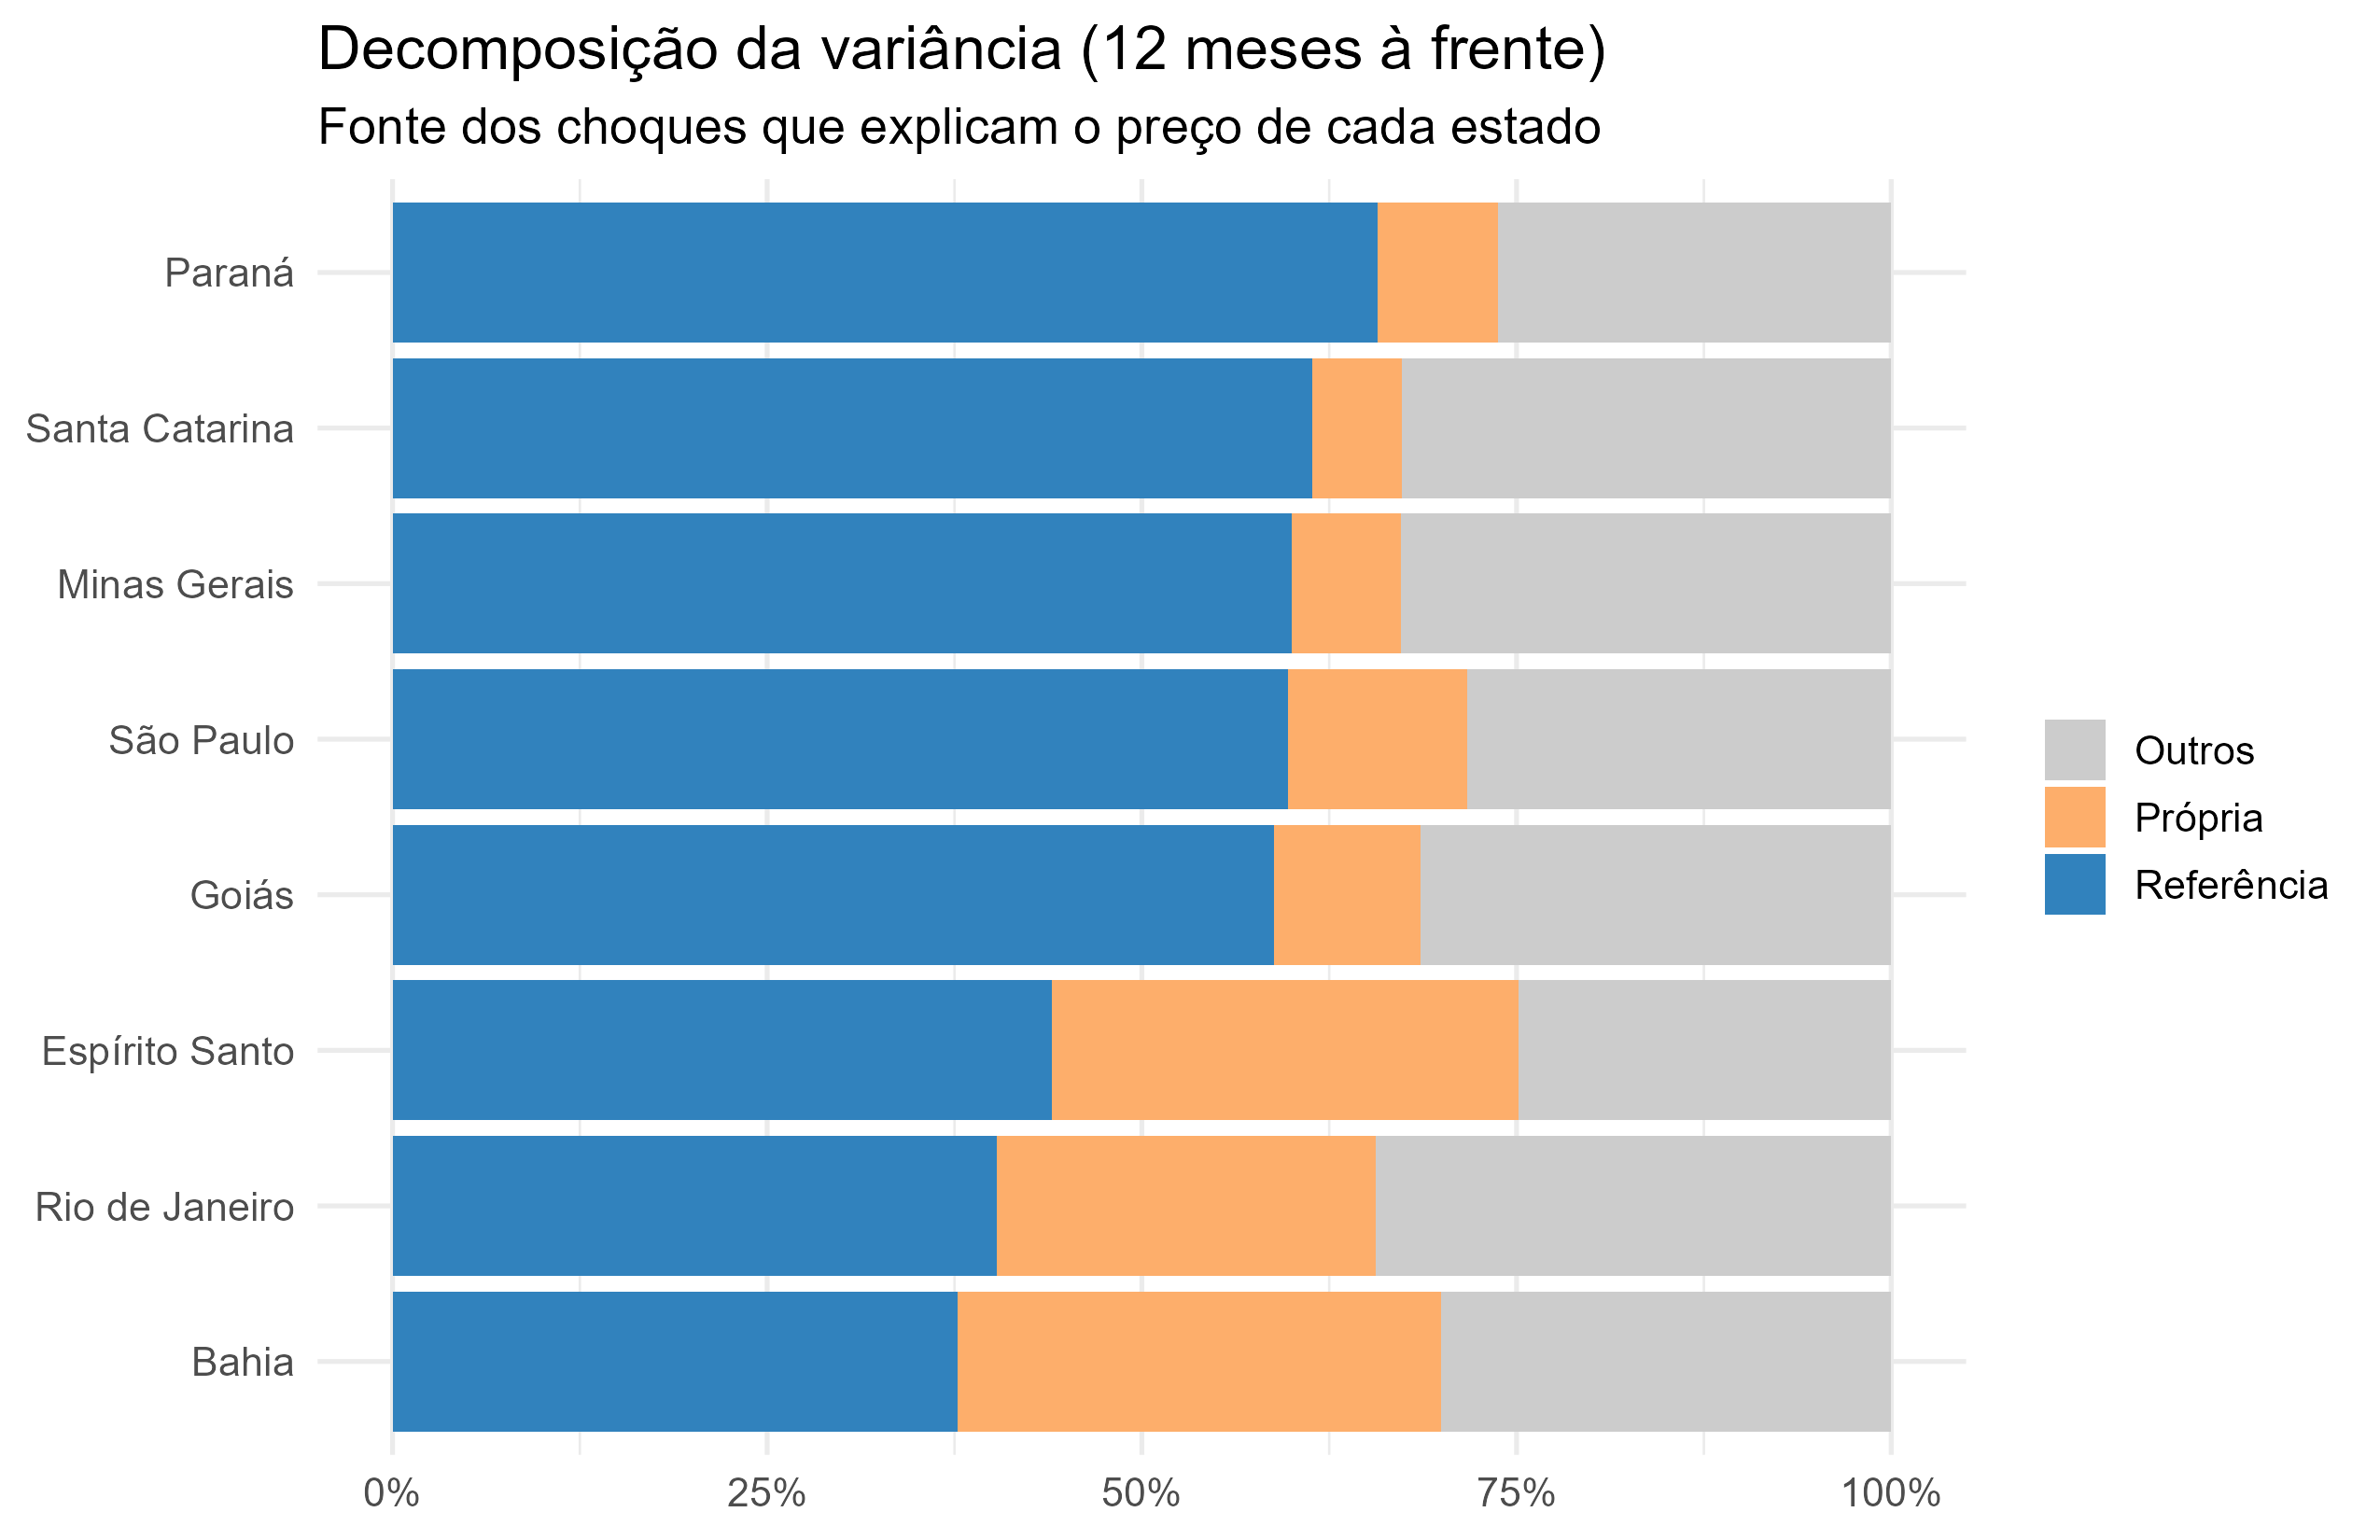
\includegraphics[width=0.8\textwidth]{fig07_fevd.png}
  \caption{Decomposição da variância do erro de previsão (12 meses): fonte dos choques
  que explicam o preço de cada estado.}
  \label{fig:fevd}
\end{figure}

\begin{table}[!h]
\centering
\caption{\label{tab:fevd}Decomposição da variância do erro de previsão a 12 meses.}
\centering
\fontsize{10}{12}\selectfont
\begin{tabular}[t]{lrrr}
\toprule
\textbf{Estado} & \textbf{\% Referência} & \textbf{\% Própria} & \textbf{\% Outros}\\
\midrule
\cellcolor{gray!10}{Bahia} & \cellcolor{gray!10}{37,7\%} & \cellcolor{gray!10}{32,2\%} & \cellcolor{gray!10}{30,0\%}\\
Espírito Santo & 44,0\% & 31,1\% & 24,9\%\\
\cellcolor{gray!10}{Goiás} & \cellcolor{gray!10}{58,8\%} & \cellcolor{gray!10}{9,8\%} & \cellcolor{gray!10}{31,4\%}\\
Minas Gerais & 60,0\% & 7,3\% & 32,7\%\\
\cellcolor{gray!10}{Paraná} & \cellcolor{gray!10}{65,7\%} & \cellcolor{gray!10}{8,0\%} & \cellcolor{gray!10}{26,2\%}\\
Rio de Janeiro & 40,3\% & 25,3\% & 34,4\%\\
\cellcolor{gray!10}{Santa Catarina} & \cellcolor{gray!10}{61,4\%} & \cellcolor{gray!10}{6,0\%} & \cellcolor{gray!10}{32,6\%}\\
São Paulo & 59,8\% & 11,9\% & 28,3\%\\
\bottomrule
\end{tabular}
\end{table}


% =====================================================================
\section{Considerações finais}
Os resultados desenham um mercado nacional de leite ao produtor fortemente integrado:
as séries são $I(1)$ e cointegradas, com elasticidades de longo prazo próximas da
unidade, correção de erro rápida (15--46\% ao mês) e transmissão majoritariamente
simétrica. Modelos de limiar (TVECM) indicam, para parte dos pares, uma banda de
não-arbitragem compatível com custos de transação. A causalidade de Granger e a
decomposição da variância apontam liderança de preços nos grandes centros produtores e na
referência nacional, com mercados periféricos mais autônomos. Tais evidências são
coerentes com um mercado espacialmente eficiente, ainda que sujeito a fricções de
transação em rotas específicas.

% =====================================================================
\begin{thebibliography}{99}
\bibitem{balke1997} Balke, N.~S.; Fomby, T.~B. (1997). Threshold cointegration.
\textit{International Economic Review}, 38(3), 627--645.
\bibitem{enders2001} Enders, W.; Siklos, P.~L. (2001). Cointegration and threshold
adjustment. \textit{Journal of Business \& Economic Statistics}, 19(2), 166--176.
\bibitem{engle1987} Engle, R.~F.; Granger, C.~W.~J. (1987). Co-integration and error
correction: representation, estimation, and testing. \textit{Econometrica}, 55(2),
251--276.
\bibitem{goodwin2001} Goodwin, B.~K.; Piggott, N.~E. (2001). Spatial market integration
in the presence of threshold effects. \textit{American Journal of Agricultural
Economics}, 83(2), 302--317.
\bibitem{granger1969} Granger, C.~W.~J. (1969). Investigating causal relations by
econometric models and cross-spectral methods. \textit{Econometrica}, 37(3), 424--438.
\bibitem{hansen2002} Hansen, B.~E.; Seo, B. (2002). Testing for two-regime threshold
cointegration in vector error-correction models. \textit{Journal of Econometrics},
110(2), 293--318.
\bibitem{johansen1988} Johansen, S. (1988). Statistical analysis of cointegration
vectors. \textit{Journal of Economic Dynamics and Control}, 12(2--3), 231--254.
\bibitem{johansen1991} Johansen, S. (1991). Estimation and hypothesis testing of
cointegration vectors in Gaussian vector autoregressive models. \textit{Econometrica},
59(6), 1551--1580.
\bibitem{meyer2004} Meyer, J.; von Cramon-Taubadel, S. (2004). Asymmetric price
transmission: a survey. \textit{Journal of Agricultural Economics}, 55(3), 581--611.
\bibitem{phillips1990} Phillips, P.~C.~B.; Ouliaris, S. (1990). Asymptotic properties of
residual based tests for cointegration. \textit{Econometrica}, 58(1), 165--193.
\bibitem{sims1980} Sims, C.~A. (1980). Macroeconomics and reality.
\textit{Econometrica}, 48(1), 1--48.
\bibitem{vct1996} von Cramon-Taubadel, S.; Loy, J.-P. (1996). Price asymmetry in the
international wheat market. \textit{Canadian Journal of Agricultural Economics}, 44(3),
311--325.
\end{thebibliography}

\end{document}
